\documentclass[12pt, a4paper]{article}
\usepackage{fullpage}
\usepackage[utf8]{inputenc}
\usepackage{natbib}
\usepackage{blindtext}
\usepackage{graphicx}
\bibliographystyle{abbrvnat}

\setlength{\parindent}{0em}
\setlength{\parskip}{1em}
\title{Title of the paper}%
\author{Markus Graf}
\begin{document}

\maketitle
\section*{The avalanche disaster from the 25th January 1689}

\begin{quote}
 It was the day named  conversion of St. Paul, at the 25 of January 1689 at 8 o'clock, when we had to feel wrath of the highest of all God, as two dry avalanches went over the community of Saas, and in which 59 People lost their lives. From the community of Saas 48 died, 5 from Conters, two from Fideris, 3 from Davos and one from Küblis.
 
The first avalanche, which went off at 8 o'clock, started outwards at Calmur in Büel, called the ``Hannen''; from that point on it took the way through the forest and through the mountain down till inside Marthels; from there to the Landquartstutz. Cruelly it tore down   forest, stables, houses, arboretums. 10 houses were destroyed, 15 People died; several were dug out alive. Two girls and an older woman for example, the woman was buried with first avalanche, the girl with the second. They were dug out not until the next day. 

After the first avalanche,  about 9 o'clock,  a good amount of friends  and neighbours were running for help because of the miserable screams and the raging church bells, its damage was not visible from Conters because of the wind and weather. They were also running from Küblis and till 12 o'clock they dug out People and livestock. At this hour another avalanche arrived. It started at Calandagrat and went down the mountain across Drumalinis, over the Barglein at Gruob, across the Landwasser, with the result that on the other side of the valley was covered with wood, 	household effects and that sort of thing. This avalanche also tore down everything in front of it. 12 houses  were destroyed, 44 People rest death or died from the consequences. Most of the rescue team was beaten down while escaping; people escaped inwards got away. Several begun to work again, others fled. At this hour a sort of people from Serneus went to help. We dug out alive five persons from a pile on youth Rudolfs Brosis house. We wish a cheerful resurrection to those who passed away to God, the Lord and a blessed the end the survivors. Many were dug out alive, many were healthy, several were injured, those I wish patience and get well. But those who lost all their belongings, those console oneself with Hiobs words of the first chapter in verse 21: And said, Naked came I out of my mother's womb, and naked shall I return thither: the lord gave, and the lord hath taken away; blessed be the name of the lord. They buried all corpses within 9 weeks, most of them were intact as they died in their beds. 

After the second avalanche several people worked till midnight and dug out people death and alive at all times. They buried first 23 bodies in the churchyard of Saas, 3 in Conters and one in Küblis. The other time 12 in Saas, and the third time 6. 

I, Daniel Jost from Conters, witnessed the events with my own eyes. I recognized the second avalanche and tried to warn them to escape inwards by shouting and whistle imploringly. Half of the people fled inwards where knocked but stayed alive, the others who fled outwards all died. I fled, was frightened and scared, I can't tell more of this event.
 -- Daniel Jost, witness of the tragedy \cite[p.~50]{hansemann1995saaser}
\end{quote}


 \citep[p.~99]{pfister2002tag}

\begin{figure}[htpb!]
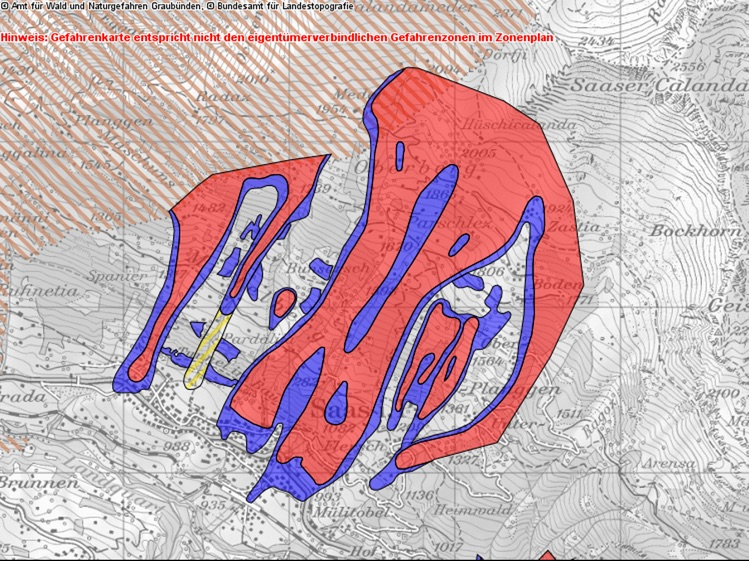
\includegraphics[width=\textwidth,natwidth=610,natheight=642]{literature/gefahrenkarte.jpg}
\caption{Map of risk for Saas im Prätigau \cite{gefahrenkarte}}
\end{figure}

\bibliography{literature}


\end{document}